%!TEX root = ../thesis.tex
% створюємо розділ
\chapter{Доведення CO-NP повноти}
\label{chap:theory}

Доведення того, що \emph{MinTSP} є coNP повною є еквівалентне доведенню
NP повноти наступної задачі:
\begin{definition}
    \emph{TSPAnotherTour: } Нехай дано повний граф $G = (V, E)$ з невід\textquotesingleємними цілими вагами
$d_{ij}$ між ребрам, та простий ланцюг C, що містить всі вершини графу G.
\par\emph{Запитання: } чи існує простий цикл D, який відвідує всі вершини G, такі, що уся
довжина шляху D в G строго менше, за загальну довжину шляху C в G?
\end{definition}

\begin{theorem}
    \emph{TSPAnotherTour є NP повною.}
\end{theorem}
\begin{proof}
\\Покажемо, що існує вирішення цієї задачі, яке працює за поліноміальний час:
просто перевіряємо, чи відвідує шлях D \emph{усі} міста та чи його довжина
строго менша за довжину даного шляху C, тому проблема знаходиться в класі NP.

\emph{Залишилось довести, що дана задача є повною в класі NP.} Для цього
побудуємо поліноміальне зведення задачі \emph{3SAT} до TSPAnotherTour.
Нехай дана формула $\phi$ в 3-КНФ з $n$ змінними $x_{1},\ldots,x_{n}$ та $m$ диз\textquotesingleюнктів
$C_{1},\ldots,C_{m}$. Ми представимо нову фіктивну змінну $z$ та добавимо її
до кожного диз\textquotesingleюнкту: $(x_{i_{1}} \vee x_{i_{2}} \vee x_{i_{3}} \vee z)$.
Отримали формулу $\phi^{z}$ в 4-КНФ, що має принаймі 1 модель.

\par Побудуємо з формули $\phi^{z}$ неорієнтований граф $G=(V, E)$
використовуючи стандартне перетворення формули в граф (як от наприклад в доведенні
NP-повноти проблеми Гамільтонівого циклу): Для кожного диз\textquotesingleюнкту ми додаємо вершину
$c_{j}$, для кожної змінної $x_{i}$ ми додаємо \emph{спеціальний} компонент.
Додаємо направлене ребро з спеціальної компоненти до вершини $c_{j}$, якщо 
$x_{i}$ з\textquotesingleявляється в $C_{j}$ як позитивна змінна. Додаємо направлене ребро
з $c_{j}$ до однієї з \emph{спеціальних} вершин, якщо $x_{i}$ з\textquotesingleявляється 
в $C_{j}$ як негативна змінна.

\parПочинаючи з верху ми можемо обійти спеціальні компоненти відповідно до
змінних $x_{1},\ldots,x_{n}$ починаючи зліва на право(встановлюючи, що $x_{i} = T$), або
справа на ліво(встановлюючи $x_{i} = F$). Отриманий орієнтований граф $G$ буде
буде містити Гамільтонів цикл тоді та тільки тоді, коли коли вхідна формула
буде мати принаймі 1 модель. 

\parДивимось на \emph{спеціальні} компоненти відповідно до фіктивної змінної
$z$. Нехай $e_{z}$ буде ребро, яке ми маємо обійти, якщо ми встановимо змінну
$z$ як істинну. 

\begin{figure}[ht]
    \centering
    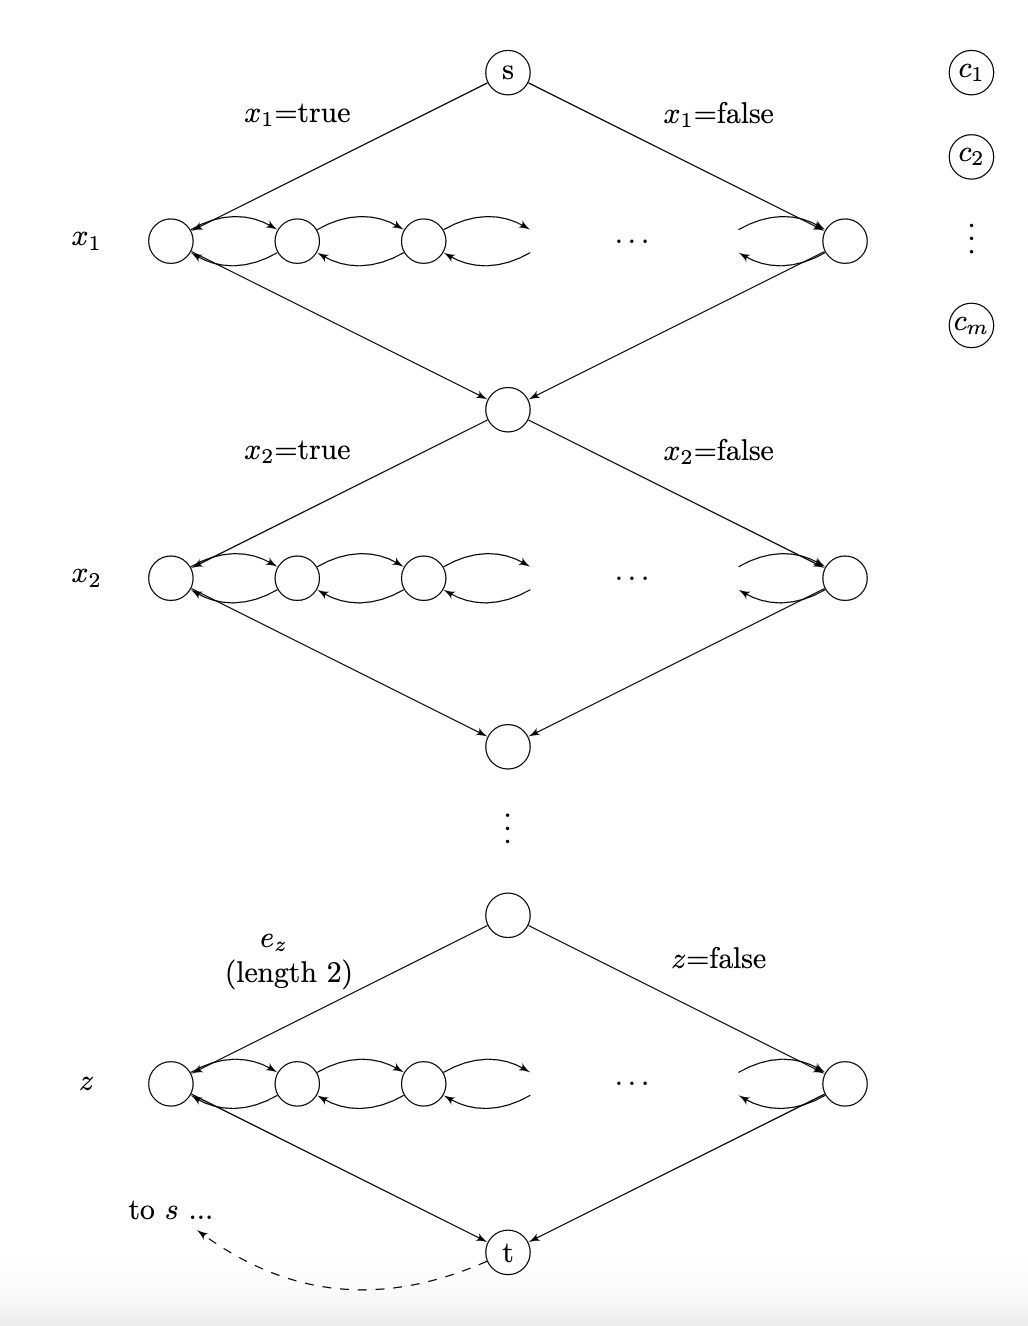
\includegraphics[scale=0.5]{Images/graph.jpg}
    \label{graph}
\end{figure}

Переробимо граф $G$ на відповідний неорієнтований граф $G\textquotesingle=(V\textquotesingle, E\textquotesingle)$
замінюючи кожну вершину $u \in V$ на 3 звязаних вершини $u_{1}, u_{2}, u_{3} \in V\textquotesingle$
і модифікуючи направлені ребра відповідно до зведення, яке використовується в доведенні
NP-повноти проблеми неорієнтованого Гамільтонівого циклу до проблеми орієнтованого Гамільтонівого
циклу: будемо використовувати $u_{1}$ як вхідне ребро $u$, та $u_{3}$ як вихідне ребро u,
тобто ми замінюємо кожне направлене ребро $(u \to v) \in E$ на $(u_{3} \to v_{1}) \in E\textquotesingle$.
Отримали, що $G\textquotesingle$ буде містити Гамільтонів цикл тоді та тільки тоді, коли G буде містити 
Гамільтонів цикл тоді та тільки тоді, коли $\phi^{z}$ буде мати принаймі 1 модель.

\parНаприкінці, переробимо граф $G\textquotesingle$ на відповідний граф для \emph{TSPAnotherTour}
змінюючи розмір всіх ребер, окрім ребра $e_{z}$, яке має довжину 2. Також, добавимо ребра, яких не
вистачає і встановимо їх довжину як 3. 
Фіктивна змінна $z$ гарантуємо нам, що ми можемо легко знайти шлях $T$:
просто обходимо спеціальні компоненти зліва на право. Коли натрапляємо на компоненту відповідну до
змінної $z$, обходимо її також зліва на право (встановлюючи, що змінна $z = T$), включаючи
усі $c_{j}$. Така побудова графу гарантуємо нам довжину усього шляху рівну точно $|V| = |V\textquotesingle|
+ 1$, всі ребра мають довжину 1, окрім ребра $e_{z}$, яке має довжину 2.
Інших шлях $D$ може мати довжину строгу меншу за $|V\textquotesingle|+1$ лише тоді, якщо 
$D$ не використовує ребро $e_{z}$. Отже, якщо він існує, ми можемо побудувати 
відповідне рішення використовуючи початкову формулу $\phi$. Також, $\phi$ буде мати модель
тоді та тільки тоді, коли існує відповідна модель для $\phi^{z}$, в якій $z=F$.
В кінці кінців, якщо існує модель для $\phi$, ми можемо легко знайти шлях $D$
довжини $|V\textquotesingle|$: просто обходити \emph{спеціальні} компоненти відповідно
до істинності змінних $x_{i}$ і обходити спеціальні компоненти, які відносяться до $z$ справа
на ліво. 
\\Отже, такий маршрут $D$ з довжиною шляху строго меншою за довжину шляху $T$ існує тоді та тільки тоді,
коли вхідна 3SAT формула має принаймі 1 модель.

\end{proof}

\begin{corollary}
    \emph{MinTSP є coNP повною. }
\end{corollary}

\section{Наявні методи розвязку}

Відомі методи розв'язання поділяють на дві групи, що можна комбінувати. 
Точні методи знаходять, маючи достатньо часу, гарантовано оптимальний шлях.
Евристичні методи знаходять, часто за коротший час, гарні розв'язки, що, в загальному випадку,
можуть бути гіршими за оптимальні. Для метричної задачі існують евристики, що знаходять за
поліноміальний час розв'язки гірші за оптимальні у 1.5—2 рази.

\begin{enumerate}
    \item Точні методи(метод гілок і меж)
    Можна знайти точний розв'язок задачі комівояжера, тобто,
    обчислити довжини всіх можливих маршрутів та обрати маршрут з найменшою довжиною.
    Однак, навіть для невеликої кількості міст в такий спосіб задача практично нерозв'язна. 
    \item Евристичні методи
    Для пришвидшення пошуку прийнятних маршрутів можна використовувати евристики, що,
    в загальному випадку, не гарантують точності знайдених розв'язків. В залежності від того,
    чи обчислює евристика новий маршрут, чи намагається покращити вже існуючий, евристики поділяють
    на конструктивні та ітеративні евристики. Крім того, відрізняють дуальні евристики, та метаевристики. 
    \item Метаевристичні методи
    Метаевристичні методи комбінують методи пошуку локальних та глобальних розв'язків у
    абстрактні стратегії евристичної оптимізації задач.
    \item Генетичні алгоритми
\end{enumerate}

\section{Ефективні розвязки задачі}

Всі ефективні методи(не використовуючи повний перебір) розвязку задачі Комівояжера грунтуються на різних евристиках.
Однак, вони знаходять не найбільш ефективний маршрут, а наближене рішення. Один з існуючих таких методів
грунтується на використані мінімальних кістякових дерев, які дають рішення з фактом апроксимації 2, і мають складність
$O(n^2 * logn)$. Ідея полягає в тому, що кожен зв'язний граф містить нижній поріг вартості його підграфа
- мінімальне кістякове дерево, і в тому, що будь-який цикл, що відвідує кожну вершину графа мінімум один раз,
може бути трансформований в оптимальний з точки зору вартості маршрут при використанні різних метрик.

\section{Цікаві, на мій погляд, речі}

За умови, $P\neq NP$ не існує алгоритму, що для деякого поліному p обчислював би такі розв'язки задачі комівояжера,
що відрізнялись би від оптимального щонайбільше на коефіцієнт $2^{p(n)}$.
Однак, існують алгоритми пошуку наближених розв'язків для метричної задачі за поліноміальний час, і
знайдений маршрут щонайбільше вдвічі (наприклад, 1.5 для алгоритму Христофіда) довший за оптимальний. 